\section{Ray/beam tracing in the isogeometric framework}
Beam tracing builds upon ray tracing and was introduced by Heckbert and Hanrahan~\cite{Heckbert1984btp}. It offers a high frequency approximation of scattering problems and has been frequently used in the BeTSSi community. In the following we investigate ray/beam tracing in the isogeoemtric framework. Again, the meshing procedure is avoided, and the ray tracing algorithm may operate directly on the CAD model.

Ray tracing approximates the solution of the Helmholtz equation~\cite{Jensen2011coa}
\begin{equation*}
	\nabla^2 p(\vec{x}) + k^2p(\vec{x}) = 0
\end{equation*}
as a ray series
\begin{equation*}
	p(\vec{x}) = \euler^{\imag\omega\tau(\vec{x})}\sum_{j=0}^\infty \frac{A_j(\vec{x}_j)}{(\imag\omega)^j}
\end{equation*}
which yields the eikonal and transport equations
\begin{align*}
\bigoh(\omega^2): &\quad |\nabla \tau|^2 = c^{-2}(\vec{x})\\
\bigoh(\omega): &\quad 2\nabla\tau\cdot\nabla A_0 +(\nabla^2\tau) A_0 = 0,\\
\bigoh(\omega^{1-j}): &\quad 2\nabla\tau\cdot\nabla A_j +(\nabla^2\tau) A_j = -\nabla^2 A_{j-1},\quad j = 1,2,\dots.
\end{align*}
Beam tracing forms an alternative to finding eigenrays. As opposed to finding eigenrays, beam tracing does not require solving the non-linear problem of finding eigenrays. 
In case of constant sound speed, $c_{\mathrm{f}}$, the ray trajectories are linear curves, and the pressure along ray $j$ is given by
\begin{equation*}
	p_j(s) = \frac{A_{0,j}}{s}\euler^{\imag k s}.
\end{equation*}
Ray/Beam tracing then reduces to finding intersection between straight lines and surfaces. The amplitude of a ray is constructed in such a way that we have energy conservation
\begin{equation*}
	\int_{\partial V_0} |p_j|^2\idiff S = \int_{\partial V_1} |p_j|^2\idiff S = \text{const},
\end{equation*}
where $\partial V_0$ and $\partial V_1$ are two reference cross sections along the beam. A beam can be constructed using linear shape functions with $s$ being the parameter along the center ray, and $n$ the normal distance from the observation point to the central ray
\begin{equation*}
	p_{\text{beam}}(s,n) = A_{\text{beam}}(s)\phi(s,n)\euler^{\imag k s},\quad \phi(s,n) = \begin{cases} \frac{W(s)-n}{W(s)} & n\leq W(s)\\
	0 & \text{else.}\end{cases}
\end{equation*}

\subsection{Beam tracing using linear shape functions}
Assuming the object under consideration is parametrized by NURBS, the control polygon bounds the domain (\Cref{Fig:boundingBox}).
\begin{figure}
	\centering
	\begin{subfigure}[t]{0.49\textwidth}
		\centering
		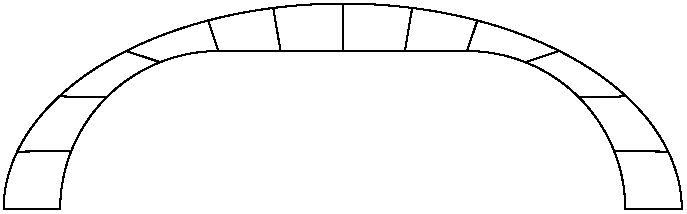
\includegraphics[scale=0.3]{../../graphics/S1/mesh3}
		\caption{The control polygon bounds the scatterer.}
		\label{Fig:boundingBox}
	\end{subfigure}%
	\hspace*{0.02\textwidth}%
	\begin{subfigure}[t]{0.49\textwidth}
		\centering
		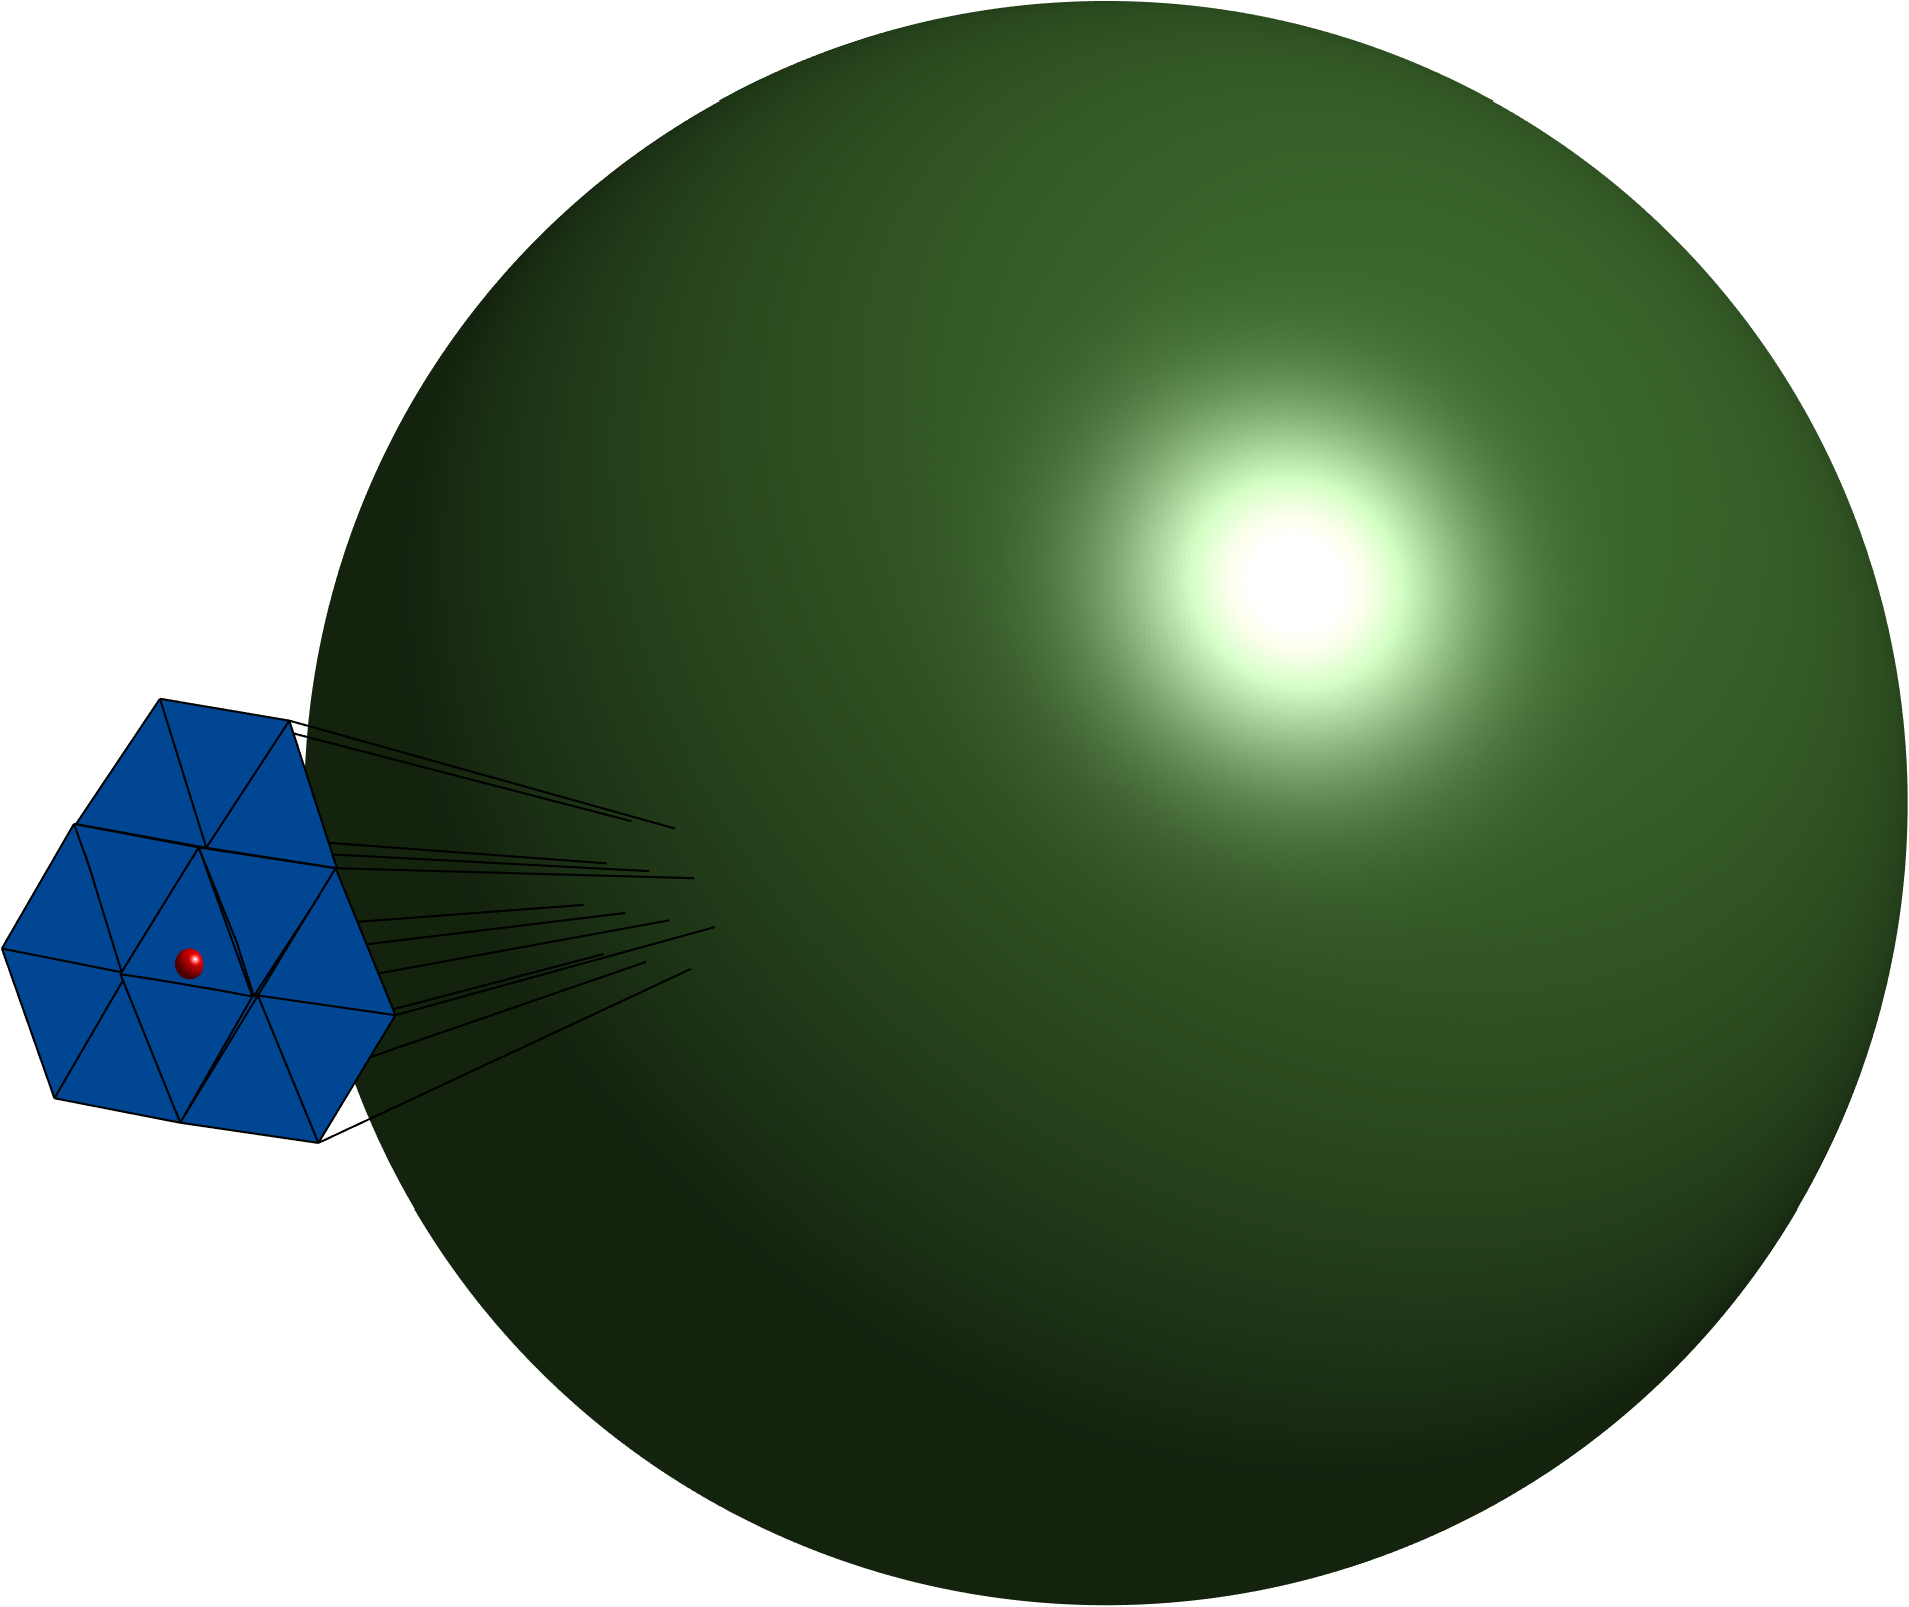
\includegraphics[scale=0.4]{../../graphics/S1/beam2}
		\caption{Three beams having support at $\vec{x}$.}
		\label{Fig:supportBeam}
	\end{subfigure}
	\caption{Preprocessing and postprocessing in beam tracing.}
\end{figure}
Projecting the control points onto a plane with normal vector given by $\vec{d}_{\mathrm{inc}}$ (direction of incidence of the plane wave), we find a polygon bounding a domain where rays can originate. The rays originate from vertices of equilateral triangles structured as a FEM 2D mesh of the projected polygon. To compute the scattered field at a given point, $\vec{x}$, first find the beams having support at this point (\Cref{Fig:supportBeam}). Let the center ray of a given beam be given by
\begin{equation*}
	\vec{r}_1(s) = \vec{x}_1 + s\vec{d}_1.
\end{equation*}
Minimization of the distance from $\vec{x}$ to center ray, $\|\vec{r}_1(s)-\vec{x}\|$, yields
\begin{equation*}
	s = (\vec{x}-\vec{x}_1)\cdot \vec{d}_1\quad\Rightarrow\quad \vec{P}_1 = \vec{x}_1 + [(\vec{x}-\vec{x}_1)\cdot \vec{d}_1]\vec{d}_1.
\end{equation*}
The boundary of the beam around $\vec{x}$ is determined by the vertices $\vec{P}_i$. These vertices are found by solving $(\vec{r}_i(s)-\vec{P}_1)\cdot \vec{d}_1 = 0$ where $\vec{r}_i(s) = \vec{x}_i + s\vec{d}_i$
\begin{equation*}
	s = \frac{(\vec{P}_1-\vec{x}_i)\cdot\vec{d}_1}{\vec{d}_i\cdot\vec{d}_1}\quad\Rightarrow\quad \vec{P}_i = \vec{x}_i + \frac{(\vec{P}_1-\vec{x}_i)\cdot\vec{d}_1}{\vec{d}_i\cdot\vec{d}_1}\vec{d}_i.
\end{equation*}
Write $\vec{x}$ in terms of barycentric coordinates 
\begin{equation*}
	\vec{x} = \vec{P}_1+\xi_2(\vec{P}_2-\vec{P}_1)+\xi_3(\vec{P}_3-\vec{P}_1)
\end{equation*}
then
\begin{equation*}
	\vec{x}\in \Delta(\vec{P}_1,\vec{P}_2,\vec{P}_3)\quad\text{if}\quad \xi_2,\xi_3\geq 0 \quad\wedge \quad\xi_2+\xi_3 \leq 1.
\end{equation*}
Solving for $\xi_2$ and $\xi_3$ yields (with $\vec{v}_1 = \vec{P}_2-\vec{P}_1$ and $\vec{v}_2 = \vec{P}_3-\vec{P}_1$)
\begin{align*}
	\xi_2 &= \frac{(\vec{v}_2\cdot\vec{v}_2)(\vec{x}-\vec{P}_1)\cdot\vec{v}_1-(\vec{v}_1\cdot\vec{v}_2)(\vec{x}-\vec{P}_1)\cdot\vec{v}_2}{(\vec{v}_1\cdot\vec{v}_1)(\vec{v}_2\cdot\vec{v}_2)-(\vec{v}_1\cdot\vec{v}_2)^2}\\
	\xi_3 &= \frac{(\vec{v}_1\cdot\vec{v}_1)(\vec{x}-\vec{P}_1)\cdot\vec{v}_2-(\vec{v}_1\cdot\vec{v}_2)(\vec{x}-\vec{P}_1)\cdot\vec{v}_1}{(\vec{v}_1\cdot\vec{v}_1)(\vec{v}_2\cdot\vec{v}_2)-(\vec{v}_1\cdot\vec{v}_2)^2}
\end{align*}
which is well defined because of Cauchy-Schwarz inequality. 

For the far field evaluations, note that the center ray goes asymptotically as
\begin{equation*}
	\vec{r}_1(s) \sim s\vec{d}_1.
\end{equation*}
Minimization of the distance from $\vec{x}$ to center ray, $\|\vec{r}_1(s)-\vec{x}\|$, yields
\begin{equation*}
	s \sim \vec{x}\cdot \vec{d}_1\quad\Rightarrow\quad \vec{P}_1 \sim (\vec{x}\cdot \vec{d}_1)\vec{d}_1.
\end{equation*}
The boundary of the beam around $\vec{x}$ is determined by the vertices $\vec{P}_i$. These vertices are found by solving $(\vec{r}_i(s)-\vec{P}_1)\cdot \vec{d}_1 = 0$
\begin{equation*}
	s \sim \frac{\vec{P}_1\cdot\vec{d}_1}{\vec{d}_i\cdot\vec{d}_1}\quad\Rightarrow\quad \vec{P}_i \sim \frac{\vec{x}\cdot\vec{d}_1}{\vec{d}_i\cdot\vec{d}_1}\vec{d}_i.
\end{equation*}
With 
\begin{equation*}
	\vec{v}_1 = \vec{P}_2-\vec{P}_1 \sim (\vec{x}\cdot \vec{d}_1)\left(\frac{\vec{d}_2}{\vec{d}_1\cdot \vec{d}_2} - \vec{d}_1\right)
\end{equation*}
and
\begin{equation*}
	\vec{v}_2 = \vec{P}_3-\vec{P}_1 \sim (\vec{x}\cdot \vec{d}_1)\left(\frac{\vec{d}_3}{\vec{d}_1\cdot \vec{d}_3} - \vec{d}_1\right)
\end{equation*}
we find
\begin{align*}
	\vec{v}_1\cdot\vec{v}_2 &\sim (\vec{x}\cdot \vec{d}_1)^2\left(\frac{\vec{d}_2\cdot\vec{d}_3}{(\vec{d}_1\cdot \vec{d}_2)(\vec{d}_1\cdot \vec{d}_3)} - 1\right)\\
	\vec{v}_1\cdot\vec{v}_1 &\sim (\vec{x}\cdot \vec{d}_1)^2\left(\frac{1}{(\vec{d}_1\cdot \vec{d}_2)^2} - 1\right)\\
	\vec{v}_2\cdot\vec{v}_2 &\sim (\vec{x}\cdot \vec{d}_1)^2\left(\frac{1}{(\vec{d}_1\cdot \vec{d}_3)^2} - 1\right).
\end{align*}
Write $\vec{x}$ in terms of barycentric coordinates 
\begin{equation*}
	\vec{x} = \vec{P}_1+\xi_2(\vec{P}_2-\vec{P}_1)+\xi_3(\vec{P}_3-\vec{P}_1)
\end{equation*}
then
\begin{equation*}
	\vec{x}\in \Delta(\vec{P}_1,\vec{P}_2,\vec{P}_3)\quad\text{if}\quad \xi_2,\xi_3\geq 0 \quad\wedge \quad\xi_2+\xi_3 \leq 1.
\end{equation*}
Solving for $\xi_2$ and $\xi_3$ yields 
\begin{align*}
	\xi_2 &= \frac{\left(\frac{1}{(\vec{d}_1\cdot \vec{d}_3)^2} - 1\right)\left(\frac{\hat{\vec{x}}\cdot\vec{d}_2}{(\hat{\vec{x}}\cdot\vec{d}_1)(\vec{d}_1\cdot \vec{d}_2)}-1\right)-\left(\frac{\vec{d}_2\cdot\vec{d}_3}{(\vec{d}_1\cdot \vec{d}_2)(\vec{d}_1\cdot \vec{d}_3)} - 1\right)\left(\frac{\hat{\vec{x}}\cdot\vec{d}_3}{(\hat{\vec{x}}\cdot\vec{d}_1)(\vec{d}_1\cdot \vec{d}_3)}-1\right)}{\left(\frac{1}{(\vec{d}_1\cdot \vec{d}_2)^2} - 1\right)\left(\frac{1}{(\vec{d}_1\cdot \vec{d}_3)^2} - 1\right)-\left(\frac{\vec{d}_2\cdot\vec{d}_3}{(\vec{d}_1\cdot \vec{d}_2)(\vec{d}_1\cdot \vec{d}_3)} - 1\right)^2}\\
	\xi_3 &= \frac{\left(\frac{1}{(\vec{d}_1\cdot \vec{d}_2)^2} - 1\right)\left(\frac{\hat{\vec{x}}\cdot\vec{d}_3}{(\hat{\vec{x}}\cdot\vec{d}_1)(\vec{d}_1\cdot \vec{d}_3)}-1\right)-\left(\frac{\vec{d}_2\cdot\vec{d}_3}{(\vec{d}_1\cdot \vec{d}_2)(\vec{d}_1\cdot \vec{d}_3)} - 1\right)\left(\frac{\hat{\vec{x}}\cdot\vec{d}_2}{(\hat{\vec{x}}\cdot\vec{d}_1)(\vec{d}_1\cdot \vec{d}_2)}-1\right)}{\left(\frac{1}{(\vec{d}_1\cdot \vec{d}_2)^2} - 1\right)\left(\frac{1}{(\vec{d}_1\cdot \vec{d}_3)^2} - 1\right)-\left(\frac{\vec{d}_2\cdot\vec{d}_3}{(\vec{d}_1\cdot \vec{d}_2)(\vec{d}_1\cdot \vec{d}_3)} - 1\right)^2}.
\end{align*}
The area of $\Delta(\vec{P}_1,\vec{P}_2,\vec{P}_3)$ is given by
\begin{equation*}
	S = \frac{1}{2}\|\vec{v}_1\times\vec{v}_2\|
\end{equation*}
which in the far field has the expression
\begin{equation*}
	S \sim \frac{1}{2}(\vec{x}\cdot\vec{d}_1)^2\left\|\frac{\vec{d}_2}{\vec{d}_1\cdot\vec{d}_2}\times\frac{\vec{d}_3}{\vec{d}_1\cdot\vec{d}_3}+\vec{d}_1\times\left(\frac{\vec{d}_2}{\vec{d}_1\cdot\vec{d}_2}-\frac{\vec{d}_3}{\vec{d}_1\cdot\vec{d}_3}\right)\right\|.
\end{equation*}
%this can be used to calculate barycentric/area coordinates (given $\vec{x}\in\Delta(\vec{P}_1,\vec{P}_2,\vec{P}_3)$)
%\begin{equation*}
%	\xi_1 = \frac{\left\|(\vec{P}_2-\vec{x})\times(\vec{P}_3-\vec{x})\right\|}{\|\vec{v}_1\times\vec{v}_2\|},\quad\xi_2 = \frac{\left\|(\vec{P}_1-\vec{x})\times(\vec{P}_3-\vec{x})\right\|}{\|\vec{v}_1\times\vec{v}_2\|}.
%\end{equation*}
The scattered field is then computed by
\begin{equation*}
	p(\vec{x}) = \sum_{j\in\{i\st \vec{x}\in B_i\}} \sqrt{\frac{E_j}{S_j}}\xi_1 \euler^{\imag k (s-s_0)}
\end{equation*}
where
\begin{equation*}
	s=\|\vec{x}-\vec{x}_1\|
\end{equation*}
and
\begin{equation*}
	E_j = \int_{\partial V_0} |p_j|^2\idiff S
\end{equation*}
corresponds to the energy of the beam $B_j$, $S_j$ is the cross-sectional area of beam $B_j$ at $\vec{x}$, $s_0$ is the phase shift and $\xi_1$ is the first barycentric coordinate at $\vec{x}$.

Exact ray reflections on a rigid sphere (radius $R_0$) from straight lines on the form
\begin{equation*}
	\vec{x}(s) = \vec{o} + \vec{d}s
\end{equation*}
can be found at (by solving $\|\vec{x}(s)\| = R_0$)
\begin{equation*}
	s = -\vec{o}\cdot \vec{d} - \sqrt{D},\quad D = (\vec{o}\cdot \vec{d})^2 + R_0^2-\|\vec{o}\|^2,
\end{equation*}
where we have reflection iff $D\geq 0$. A ray reflecting at a surface point with normal vector $\vec{n}$ has incident direction ($\vec{d}_{\mathrm{i}}$) and reflected direction ($\vec{d}_{\mathrm{r}}$) related by
\begin{equation*}
	\vec{d}_{\mathrm{r}} = \vec{d}_{\mathrm{i}} - 2(\vec{d}_{\mathrm{i}}\cdot\vec{n})\vec{n}
\end{equation*}
with $\|\vec{d}_{\mathrm{r}}\| = \|\vec{d}_{\mathrm{i}}\| = \|\vec{n}\| = 1$.
\begin{figure}
	\centering
	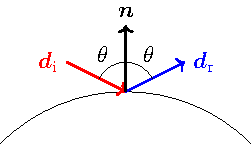
\includegraphics{../../LaTeX/createFigures/TikzFigures/raytracing_PhD/specularReflection}
	\caption{\textbf{Ray tracing}: \textit{The law of reflection} states that the angle of incidence is equal to the angle of reflection.}
\end{figure}

Let the incident wave $p_{\mathrm{inc}}(\vec{x}) = P_{\mathrm{inc}}\euler^{\imag k \vec{d}_{\mathrm{inc}}\cdot\vec{x}}$ at $\vec{x}_1 = R_0\vec{e}_{\mathrm{x}}$ be represented by a beam with circular cross section with radius $\delta$ (where $\vec{d}_{\mathrm{inc}}=-\vec{e}_{\mathrm{x}}$).
Then, $E = \int_{\partial V_0} |p_{\mathrm{inc}}|^2\idiff S = |P_{\mathrm{inc}}|^2\pi\delta^2$.
Based on the previous formulas, we find (see \Cref{Fig:asymptotic})
\begin{figure}
	\centering
	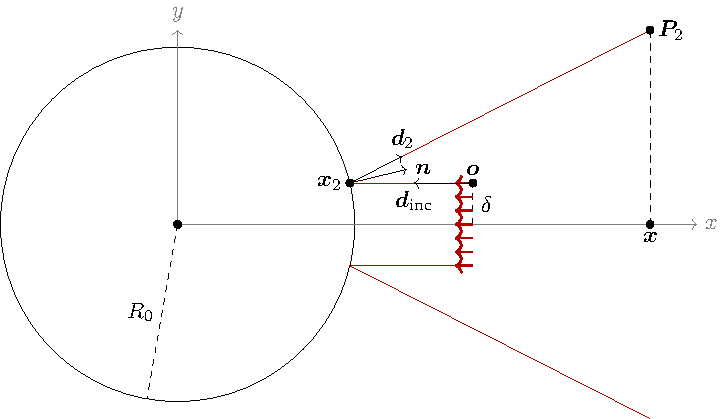
\includegraphics{../../LaTeX/createFigures/TikzFigures/raytracing_PhD/asymptotic}
	\caption{Computation of exact beam scattering solution.}
	\label{Fig:asymptotic}
\end{figure}%
\begin{align*}
	\vec{x}_2 &= \sqrt{R_0^2-\delta^2}\vec{e}_{\mathrm{x}}+\delta\vec{e}_{\mathrm{y}}\\
	\vec{d}_2 &= \left(1-2\left(\frac{\delta}{R_0}\right)^2\right)\vec{e}_{\mathrm{x}}+2\frac{\delta}{R_0}\sqrt{1-\left(\frac{\delta}{R_0}\right)^2}\vec{e}_{\mathrm{y}}\\
	\vec{P}_2 &= \vec{x} + \frac{\delta R_0^2-2\|\vec{x}\|\delta\sqrt{R_0^2-\delta^2}}{2\delta^2-R_0^2}\vec{e}_{\mathrm{y}}.
\end{align*}
The cross-section area of the beam at $\vec{x}$ is then
\begin{equation*}
	S_j = \pi\|\vec{P}_2-\vec{x}\|^2 = \pi\left(\frac{\delta R_0^2-2\|\vec{x}\|\delta\sqrt{R_0^2-\delta^2}}{2\delta^2-R_0^2}\right)^2.
\end{equation*}
The far field backscattered pressure is found by considering the limit $\|\vec{x}\|\to\infty$
\begin{equation*}
	p_0(\hat{\vec{x}}) = \frac{|P_{\mathrm{inc}}|}{2\sqrt{R_0^2-\delta^2}}(R_0^2-2\delta^2)\euler^{-2\imag k R_0}.
\end{equation*}
If we finally consider the limit $\delta\to 0$ we find
\begin{equation*}
	p_0(\hat{\vec{x}}) = \frac{|P_{\mathrm{inc}}|R_0}{2}\euler^{-2\imag k R_0}
\end{equation*}
which is the exact expression for rigid scattering on a sphere using the Kirchhoff approximation (investigated in Paper IV). This gives the target strength
\begin{equation*}
	\TS = 20\log_{10}\left(\frac{R_0}{2}\right)
\end{equation*}
which is the asymptotic limit of the analytic solution as $k\to\infty$~\cite{Fillinger2014aen}.

As can be seen from~\Cref{Fig:S1_sweep3,Fig:S1_sweep2,Fig:S1_sweep1}, beam approximation increase in accuracy as a function of the number of initial beams (geometry approximation), $N$, and increase in accuracy as a function of frequency (for sufficiently high $N$), but loses accuracy from the plane wave approximation for high frequencies at a fixed $N$. This is very similar to corresponding simulations using Kirchhoff approximation investigated in paper IV. The geometric approximation can be improved by adapting the beams for the incident wave and splitting beams at edge reflections. As the raytracing part is independent of frequency, frequency sweep calculations are very efficient using ray/beam tracing. In~\Cref{Fig:BI_1,Fig:BI_2,Fig:BI_3} it can clearly be seen that the ability to model forward scattering using ray/beam tracing is lacking.
\begin{figure}
	\centering
	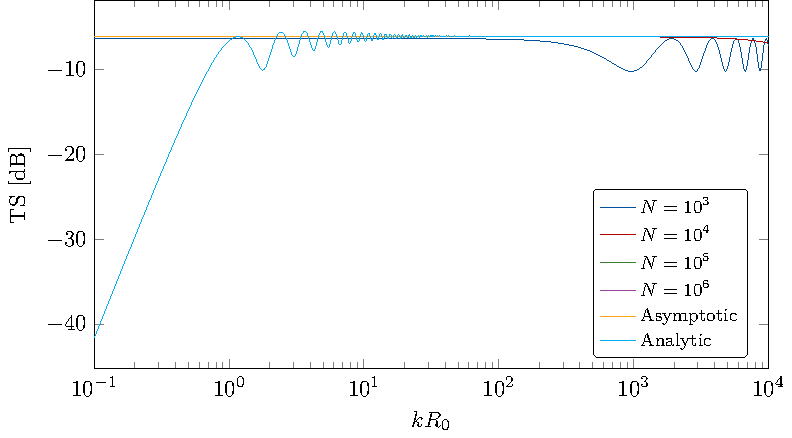
\includegraphics[width=\textwidth]{../../LaTeX/createFigures/TikzFigures/raytracing_PhD/S1_sweep_3}
	\caption{\textbf{Frequency sweep of rigid sphere}: The target strength is plotted against the dimensionless wave number.}
	\label{Fig:S1_sweep3}
\end{figure}
\begin{figure}
	\centering
	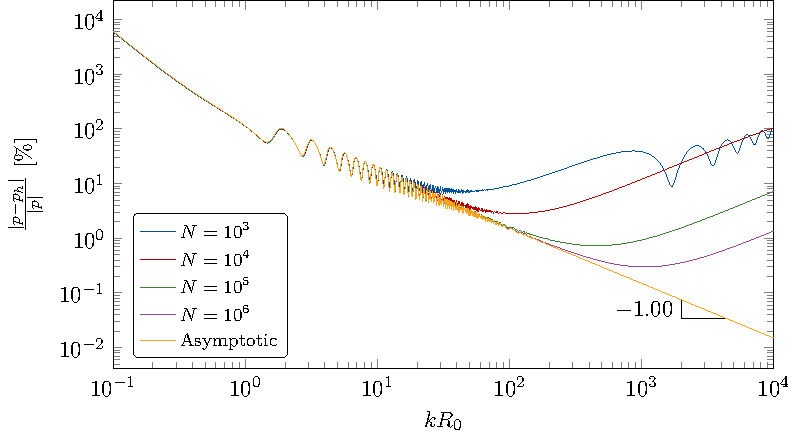
\includegraphics[width=\textwidth]{../../LaTeX/createFigures/TikzFigures/raytracing_PhD/S1_sweep_2}
	\caption{\textbf{Frequency sweep of rigid sphere}: The relative error (of the far field) is plotted against the dimensionless wave number.}
	\label{Fig:S1_sweep2}
\end{figure}
\begin{figure}
	\centering
	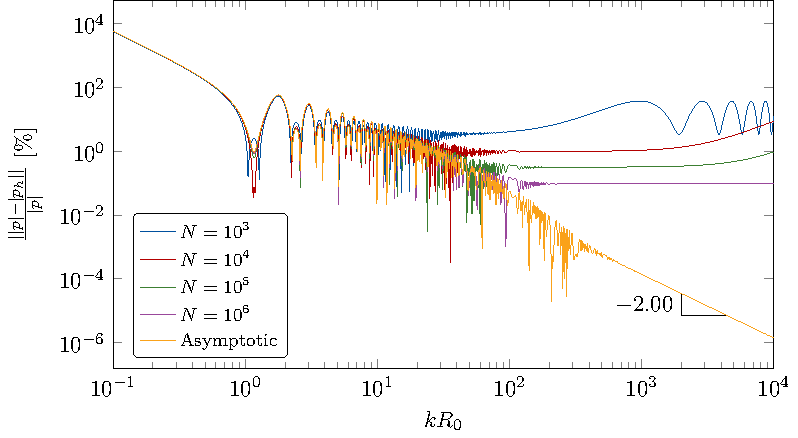
\includegraphics[width=\textwidth]{../../LaTeX/createFigures/TikzFigures/raytracing_PhD/S1_sweep_1}
	\caption{\textbf{Frequency sweep of rigid sphere}: The relative absolute error (of the far field) is plotted against the dimensionless wave number.}
	\label{Fig:S1_sweep1}
\end{figure}
\begin{figure}
	\centering
	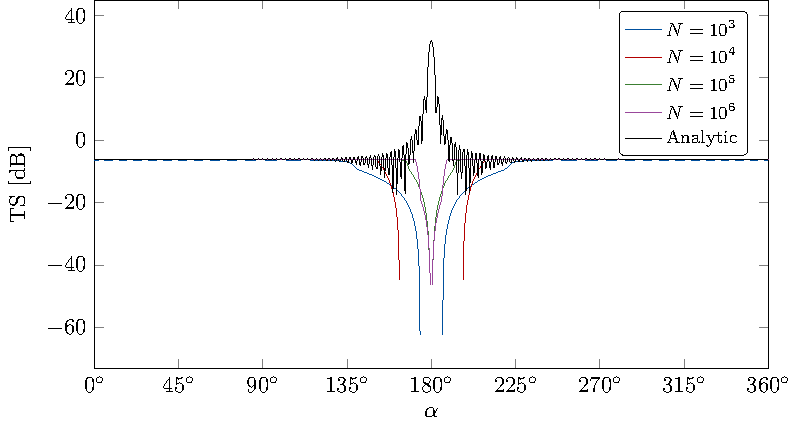
\includegraphics[width=\textwidth]{../../LaTeX/createFigures/TikzFigures/raytracing_PhD/BI_1}
	\caption{\textbf{Bistatic scattering of rigid sphere}: The target strength is plotted against the aspect angle at $f=\SI{20}{kHz}$.}
	\label{Fig:BI_1}
\end{figure}
\begin{figure}
	\centering
	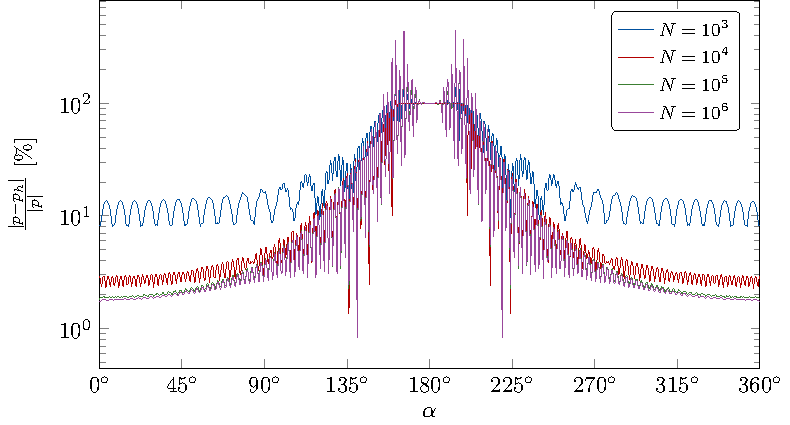
\includegraphics[width=\textwidth]{../../LaTeX/createFigures/TikzFigures/raytracing_PhD/BI_2}
	\caption{\textbf{Bistatic scattering of rigid sphere}: The relative error (of the far field) is plotted against the aspect angle at $f=\SI{20}{kHz}$.}
	\label{Fig:BI_2}
\end{figure}
\begin{figure}
	\centering
	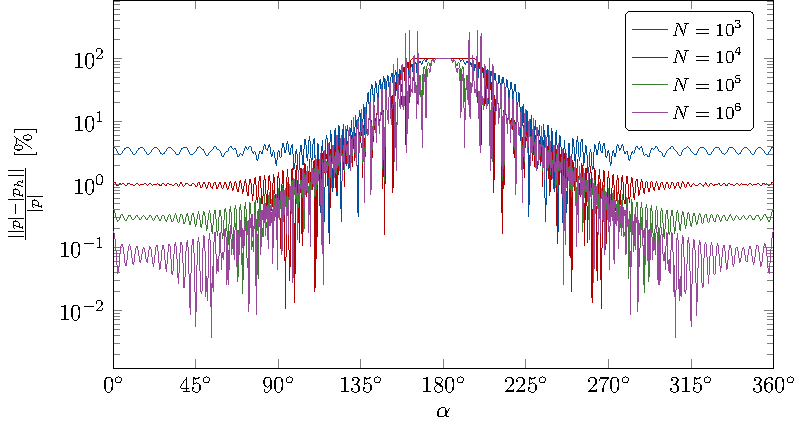
\includegraphics[width=\textwidth]{../../LaTeX/createFigures/TikzFigures/raytracing_PhD/BI_3}
	\caption{\textbf{Bistatic scattering of rigid sphere}: The relative absolute error (of the far field) is plotted against the aspect angle at $f=\SI{20}{kHz}$.}
	\label{Fig:BI_3}
\end{figure}

\subsection{Ray tracing in the isogeometric framework}
Usually the scatterer is tessellated with plane facets at which ray reflection can be trivially computed. The problem with this procedure is identical to the same approach using Kirchhoff approximation. Namely frequency dependent memory consumption and accuracy. The isogeometric framework resolves both of these issues by computing the reflections directly on the CAD-model, which in most cases can be assumed to be represented by NURBS. Additionally, IGA avoids the tesselation step entirely. However, widespread use of ray tracing using NURBS is lacking due to algebraic complexity~\cite{Martin2000prt}.

A ray tracing algorithm is presented by Martin et al.~\cite{Martin2000prt}. The algorithm first finds the intersections of the rays and a set of axis-aligned bounding boxes (see \Cref{Fig:M3_M3}).
\begin{figure}
	\centering
	\begin{subfigure}[t]{\textwidth}
		\centering
		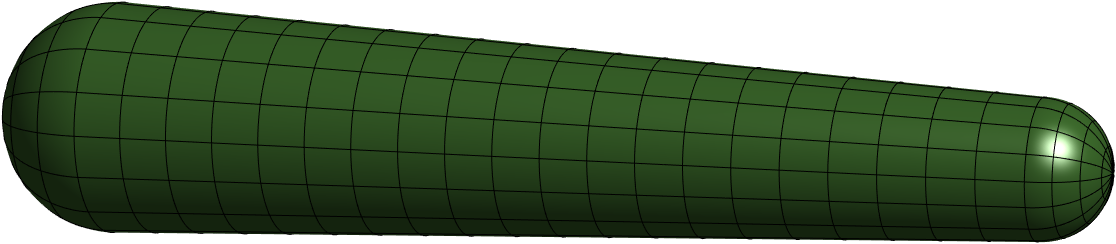
\includegraphics[scale=0.3]{../../graphics/M3/M3_M3_1}
	\end{subfigure}%
	
	\begin{subfigure}[t]{\textwidth}
		\centering
		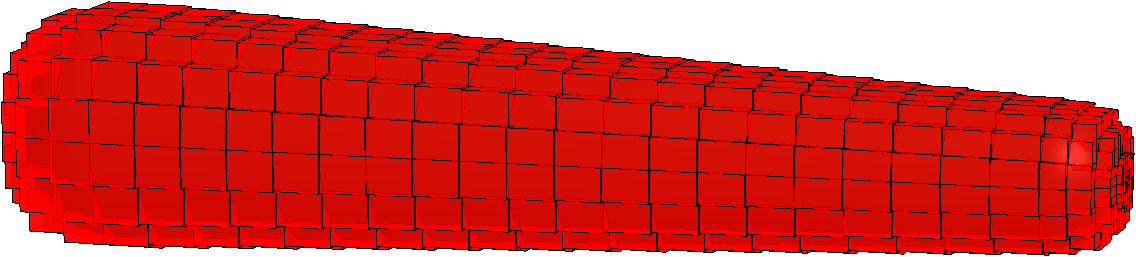
\includegraphics[scale=0.3]{../../graphics/M3/M3_M3_3}
	\end{subfigure}
	\caption{Uniform refinements gives a basis for the bounding boxes.}
	\label{Fig:M3_M3}
\end{figure}
Then for each box hit, root finding is iteratively applied (using Newton iteration) until a convergence or a divergence criterion is met. As a preprocessing step the control mesh is flattened using refinement. This step is important to obtain a good initial guess for the Newton iterations. Moreover, it reduces the chance of multiple roots in a sub-patch. This new refinement forms a basis for the bounding volume hierarchy. Note that the refined mesh data is only needed in this initial step. Flattening means refining the mesh such that each element satisfies some flatness criteria. More advanced adaptive method could be utilized. Especially local refinement methods. Martin et al.~\cite{Martin2000prt} consider a heuristic tensor product refinement strategy based on the curvature and the arclength. For each knot span, consider the number of new knots to be added is given by
\begin{equation*}
	n = C\cdot\max_{\xi\in[\xi_i,\xi_{i+1})}\{\operatorname{curvature}(\vec{X(\xi)})\}\cdot\underset{\xi\in[\xi_i,\xi_{i+1})}{\operatorname{arclength}}(\vec{X(\xi)})^{3/2}
\end{equation*}
where $C$ is a user defined parameter to control fineness. Several estimates are involved in calculating these quantities, including polynomial estimation of rational curves (NURBS-curves). In the $\xi$-direction, the number $n$ is computed for each non-empty knot span $[\eta_{j+1},\eta_j)$, such that the final number of knots to be added in $[\xi_{i+1},\xi_i)$ is the maximum of these numbers. This procedure is repeated in the $\eta$-direction of the tensor product mesh. The inserted knots are spaced uniformly in each sub interval. The final step of the flattening procedure is to duplicate the knots in the knot vector such that each knot is repeated $p$ times. The control points for each element then forms a basis for its bounding box.

The empirical parameter $C$ must be carefully chosen by the user. To small, and it can result in failure in the root finding process. To large, and the bounding volume hierarchy becomes large and computationally expensive. The hierarchy is built based upon the created bounding boxes: the leaves. These leaves are used to provide initial guess for the Newton iteration (midpoint in the element). The root and internal nodes of the tree will contain larger volumes which bounds portions of the underlying surface. The tree is formed by sorting the volumes according to the axis direction which has greatest extent across the bounding volumes, splitting the data in half, and repeating the process.

To ensure that the resulting root, $\vec{P}$, obtained by Newton iterations lie on the line, $\vec{r}(s) = \vec{o}+s\vec{d}$, the following projection is made
\begin{equation*}
	s = (\vec{P}-\vec{o})\cdot\vec{d}
\end{equation*}
Self-intersection can be avoided by a requirement that the new ray has traveled a minimum distance.

As for the sphere, the exact beams may be computed for the BeTSSi model 3. The monostatic target strength in the $xy$-plane as a function of the azimuth angle $\varphi$ is 
\begin{equation*}
	\TS = \begin{cases}
		 20\log_{10}\left(\frac{R_{\mathrm{o}2}}{2}\right) & 0\leq\varphi<\varphi_{\mathrm{max}}\\
		 \infty & \varphi = \phi_{\mathrm{max}}\\
		 20\log_{10}\left(\frac{R_{\mathrm{o}1}}{2}\right) & \varphi_{\mathrm{max}}<\varphi\leq\PI
	\end{cases}
\end{equation*}
where~\cite[p. 108]{Venas2015iao}
\begin{equation*}
	\varphi_{\mathrm{max}} = \frac{\pi}{2}-\tan^{-1}\left(\frac{R_{\mathrm{o}1}-R_{\mathrm{o}2}}{L-R_{\mathrm{o}1}-R_{\mathrm{o}2}}\right) = 1.522054475 = \ang{87.20729763}.
\end{equation*}
In~\Cref{Fig:M3_MS} a comparison is made with the beam tray tracing algorithm, the Kirchhoff algorithm (paper IV) and a reference solution created by IGABEM (paper III). The ray tracing procedure fails to obtain accurate results for the far field from the straight sections of the geometry as opposed to the Kirchhoff approximation. On the other hand, the Kirchhoff approximation (based on a simple physical optics approximation) does not model multiple reflections. A remedy for this is to use the Kirchhoff approximation based on the rays leaving the scatterer.
\begin{figure}
	\centering
	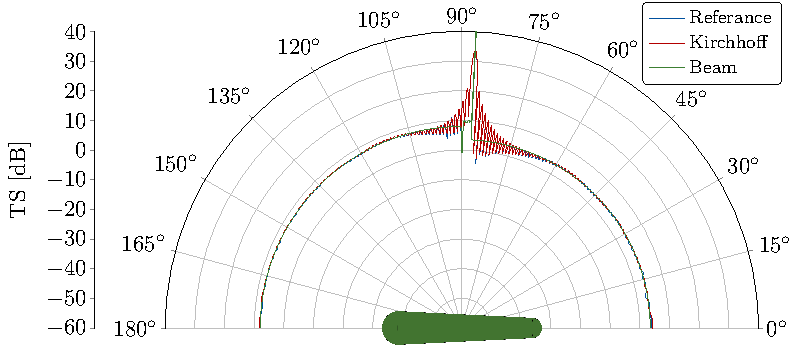
\includegraphics[width=\textwidth]{../../LaTeX/createFigures/TikzFigures/raytracing_PhD/M3_MS_4}
	\caption{Scattering on BeTSSi model 3 at $\SI{1}{kHz}$.}
	\label{Fig:M3_MS}
\end{figure}

\subsection{Computation of reflection and transmission coefficients}
For thin elastic layers, rigid boundary conditions perform poorly even for the high frequency spectrum ($f \sim \SI{10}{kHz}$). A ray hitting a surface should be divided into a reflected ray and a transmitted ray. Computation of the transmission and reflection coefficient is then necessary. The steps are presented in the following based on the work of Brekhovskikh~\cite{Brekhovskikh2012wil}.
\begin{figure}
	\centering
	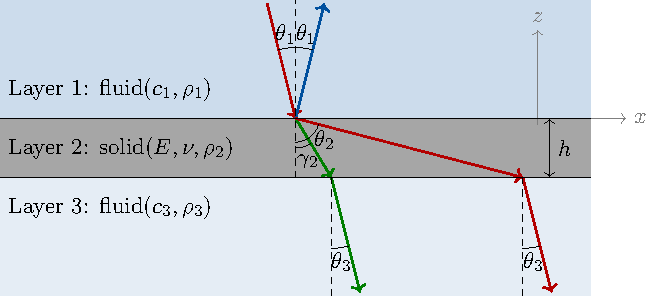
\includegraphics{../../LaTeX/createFigures/TikzFigures/raytracing_PhD/Snell}
	\caption{The incident wave is both reflected and transmitted (into longitudinal and transverse waves) through a solid infinitely large plate.}
\end{figure}

In the solid layer we not only have longitudinal waves, but also transverse waves. For any smooth surface where reflection can be defined, the scatterer can locally be approximated by a plane surface. The transmission and reflection coefficients is then computed on an infinite elastic plate. Without loss of generality the (plane) wave fronts is assumed to lie in the $xz$-plane and the layers are normal to the $z$-axis.
At each interface we require continuity of displacement and pressure (details in paper I)
\begin{equation*}
	\rho_{\mathrm{f}} \omega^2 u_i n_i - \pderiv{p_{\mathrm{tot}}}{n} = 0,\quad\sigma_{ij}n_i n_j + p_{\mathrm{tot}} = 0
\end{equation*}
which in our case is equivalent with 
\begin{equation}\label{Eq:BCs}
	\rho_{\mathrm{f}} \omega^2 u_z - \pderiv{p_{\mathrm{tot}}}{z} = 0,\quad
	\left(K-\frac{2G}{3}\right)\pderiv{u_{\mathrm{x}}}{x} + \left(K+\frac{4G}{3}\right)\pderiv{u_{\mathrm{z}}}{z} + p_{\mathrm{tot}} = 0.
\end{equation}
Here, $p_{\mathrm{tot}} = p_1 + p_{\mathrm{inc}}$ for $z > h$ (layer 1) and $p_{\mathrm{tot}} = p_2$ for $z < 0$ (layer 3) where $p_{\mathrm{inc}} = P_{\mathrm{inc}}\euler^{\imag k_1(x\sin\theta_1 - z\cos\theta_1)}$. The exterior traction vector, $\vec{T}$, has components
\begin{equation*}
	T_i = \sigma_{ij}n_j
\end{equation*}
That is, $\vec{T} = \sigma_{13}\vec{e}_{\mathrm{x}} + \sigma_{23}\vec{e}_{\mathrm{y}} + \sigma_{33}\vec{e}_{\mathrm{z}}$. For our case the tangential traction free boundary conditions are given by
\begin{equation*}
	\sigma_{13} = 0\quad\text{and}\quad \sigma_{23} = 0,
\end{equation*}
which is equivalent with
\begin{equation}\label{Eq:tractionFreeBC}
	\pderiv{u_{\mathrm{x}}}{z} + \pderiv{u_{\mathrm{z}}}{x} = 0\quad\text{and}\quad \pderiv{u_{\mathrm{z}}}{y} + \pderiv{u_{\mathrm{y}}}{z} = 0.
\end{equation}
The solution of the general Navier equation
\begin{equation*}
	G\nabla^2\vec{u}+\left(K+\frac{G}{3}\right)\nabla(\nabla \cdot\vec{u}) +\rho_{\mathrm{s}}\omega^2\vec{u} = \zerovec
\end{equation*}
can be written on the form
\begin{equation*}
	\vec{u} = \nabla\phi + \nabla\times\vec{\psi}.
\end{equation*}
In our special case we have (setting $\vec{\psi} = \psi\vec{e}_{\mathrm{y}}$)
\begin{equation*}
	u_{\mathrm{x}} = \pderiv{\phi}{x} - \pderiv{\psi}{z},\quad u_{\mathrm{y}} = 0,\quad u_{\mathrm{z}} = \pderiv{\phi}{z} + \pderiv{\psi}{x}
\end{equation*}
$\phi$ and $\psi$ are called the potentials for the longitudinal and transverse waves, respectively. These potentials satisfy the Helmholtz equation
\begin{equation*}
	\nabla^2\phi + a^2\phi = 0\quad\text{and}\quad \nabla^2\psi + b^2\psi = 0
\end{equation*}
where
\begin{equation*}
	a=\frac{\omega}{c_{\mathrm{s},1}},\quad b=\frac{\omega}{c_{\mathrm{s},2}},\quad c_{\mathrm{s},1} = \sqrt{\frac{3K+4G}{3\rho_{\mathrm{s}}}},\quad c_{\mathrm{s},2} = \sqrt{\frac{G}{\rho_{\mathrm{s}}}}.
\end{equation*}
The pressure in the fluids also solve the Helmholtz equation
\begin{equation*}
	\nabla^2 p_1 + k_1^2p_1 = 0\quad\text{and}\quad \nabla^2p_2 + k_2^2p_2 = 0
\end{equation*}
where
\begin{equation*}
	k_1=\frac{\omega}{c_{\mathrm{f},1}}\quad\text{and}\quad k_2=\frac{\omega}{c_{\mathrm{f},2}}.
\end{equation*}
We look for solutions on the form
\begin{align*}
	\phi &= A_{\upphi}\euler^{\imag (a_{\mathrm{x}} x + a_{\mathrm{z}}z)}\\
	\psi &= A_{\uppsi}\euler^{\imag (b_{\mathrm{x}} x + b_{\mathrm{z}}z)}\\
	p_1 &= A_1\euler^{\imag (k_{1\mathrm{x}} x + k_{1\mathrm{z}}z)}\\
	p_2 &= A_2\euler^{\imag (k_{2\mathrm{x}} x + k_{2\mathrm{z}}z)}
\end{align*}
where
\begin{align*}
	a^2 &= a_{\mathrm{x}}^2 + a_{\mathrm{z}}^2\\
	b^2 &= b_{\mathrm{x}}^2 + b_{\mathrm{z}}^2\\
	k_1^2 &= k_{1\mathrm{x}}^2 + k_{1\mathrm{z}}^2\\
	k_2^2 &= k_{2\mathrm{x}}^2 + k_{2\mathrm{z}}^2.
\end{align*}
The traction free boundary conditions applied to the potentials $\phi$ and $\psi$ are
\begin{equation*}
	\ppderiv{\phi}{z}{x} - \pderiv[2]{\psi}{z} + \ppderiv{\phi}{x}{z} + \pderiv[2]{\psi}{x} = 0.
\end{equation*}
Insertion yields
\begin{equation*}
	-2a_{\mathrm{x}} a_{\mathrm{z}} \phi - \left(b_{\mathrm{x}}^2-b_{\mathrm{z}}^2\right)\psi = 0
\end{equation*}
which evaluated at $z = 0$ (upper boundary of solid) gives
\begin{equation*}
	b_{\mathrm{x}} = a_{\mathrm{x}}
\end{equation*}
Evaluation of the other boundary conditions in a similar fashion yield
\begin{equation*}
	a_{\mathrm{x}} = k_{1\mathrm{x}} = k_{2\mathrm{x}} = k_1\sin\theta_1.
\end{equation*}
By writing
\begin{equation*}
	a_{\mathrm{x}} = a\sin\theta_2,\quad b_{\mathrm{x}} = b\sin\gamma_2,\quad k_{1\mathrm{x}} = k_1\sin\theta_1,\quad k_{2\mathrm{x}} = k_2\sin\theta_3
\end{equation*}
we obtain Snell's law
\begin{equation*}
	a\sin\theta_2 = b\sin\gamma_2 = k_1\sin\theta_1 = k_2\sin\theta_3.
\end{equation*}
We have
\begin{align*}
	a_{\mathrm{z}} &= \pm\sqrt{a^2-a_{\mathrm{x}}^2}\qquad
	b_{\mathrm{z}} = \pm\sqrt{b^2-b_{\mathrm{x}}^2}\\
	k_{1\mathrm{z}} &= \pm\sqrt{k_1^2-k_{1\mathrm{x}}^2}\qquad
	k_{2\mathrm{z}} = \pm\sqrt{k_2^2-k_{2\mathrm{x}}^2}
\end{align*}
so since we require no waves to originate from infinity for $p_1$ and $p_2$, then $k_{1\mathrm{x}}>0$ and $k_{2\mathrm{x}}<0$.
The solution may thus be written as 
\begin{align*}
	\phi &= A_{\upphi}^{(1)}\euler^{\imag a(x\sin\theta_2 + z\cos\theta_2)} + A_{\upphi}^{(2)}\euler^{\imag a(x\sin\theta_2 - z\cos\theta_2)}\\
	\psi &= A_{\uppsi}^{(1)}\euler^{\imag b(x\sin\gamma_2 + z\cos\gamma_2)} + A_{\uppsi}^{(2)}\euler^{\imag b(x\sin\gamma_2 - z\cos\gamma_2)}\\
	p_1 &= A_1\euler^{\imag k_1(x\sin\theta_1 + z\cos\theta_1)}\\
	p_2 &= A_2\euler^{\imag k_2(x\sin\theta_3 - z\cos\theta_3)}.
\end{align*}
Insertion of these expressions into the boundary conditions (\Cref{Eq:BCs,Eq:tractionFreeBC}) evaluated at $z=0$ and $z=-h$ yields a linear system of equations
\begin{equation*}
	\vec{H} \vec{C} = \vec{D}
\end{equation*}
where
\begin{equation*}\resizebox{\textwidth}{!}{$
\vec{H} =
\begin{bmatrix} 
-{\frac {k_1\cos \theta_1}{\rho_{\mathrm{f,1}}{\omega}^{2}}}&a\cos \theta_2 &-a\cos \theta_2 &b\sin \gamma_2 &b\sin \gamma_2&0\\ 
1&a^2 \left( -K-G \left(\frac13 + \cos 2\theta_2\right)  \right) & a^2 \left( -K-G \left(\frac13 + \cos 2\theta_2\right)  \right) &-G b^2\sin 2\gamma_2 &G b^2\sin 2\gamma_2 &0\\ 
0&- a^2\sin 2\theta_2 &a^2\sin 2\theta_2 & b^2\cos 2\gamma_2 & b^2\cos 2\gamma_2 &0\\ 
0&- a^2 \euler^{-\imag ah\cos \theta_2 }\sin 2\theta_2& a^2 \euler^{\imag ah\cos \theta_2 }\sin 2\theta_2 & b^2 \euler^{-\imag bh\cos \gamma_2}\cos 2\gamma_2& b^2 \euler^{\imag bh\cos \gamma_2}\cos 2\gamma_2 & 0 \\ 
0&a \euler^{-\imag ah\cos \theta_2 }\cos \theta_2 &-a \euler^{\imag ah\cos \theta_2 }\cos \theta_2 & b\euler^{-\imag bh\cos \gamma_2}\sin \gamma_2 & b\euler^{\imag bh\cos \gamma_2}\sin \gamma_2 & \frac { k_2\euler^{\imag k_2h\cos \theta_3 }\cos \theta_3}{\rho_{\mathrm{f,2}}{\omega}^{2}}\\ 
0& a^2 \left( -K-G \left(\frac13 +  \cos 2\theta_2 \right)  \right) {\euler^{-\imag ah\cos \theta_2 }}& a^2 \left( -K-G \left( \frac13+\cos 2\theta_2 \right) \right) {\euler^{\imag ah\cos \theta_2 }}&-G b^2 \euler^{-\imag bh\cos \gamma_2}\sin 2\gamma_2&G b^2 \euler^{\imag bh\cos \gamma_2}\sin 2\gamma_2&  \euler^{\imag k_2h\cos \theta_3}
\end{bmatrix}
$}
\end{equation*}
and
\begin{equation*}
\vec{C} = 
\begin{bmatrix}
	A_1\\
	A_\upphi^{(1)}\\
	A_\upphi^{(2)}\\
	A_\uppsi^{(1)}\\
	A_\uppsi^{(2)}\\
	A_2
\end{bmatrix},\qquad
\vec{D} = 
\begin{bmatrix} 
-\frac{P_{\mathrm{inc}}k_1\cos\theta_1}{\rho_{\mathrm{f,1}}{\omega}^{2}}\\ 
-P_{\mathrm{inc}}\\
0\\ 
0\\ 
0\\
0
\end{bmatrix}.
\end{equation*}
Solving this system, we obtain the following expressions for the reflection coefficient $R$ and transmission coefficient $T$
\begin{align*}
	R =\frac{p_1\vert_{x=0,z=0}}{P_{\mathrm{inc}}} = \frac{A_1}{P_{\mathrm{inc}}} &= \frac{M(Z_{\mathrm{f},2}-Z_{\mathrm{f},1}) + \imag\left[\left(M^2-N^2\right)Z_{\mathrm{f},2}+Z_{\mathrm{f},1}\right]}{M(Z_{\mathrm{f},2}+Z_{\mathrm{f},1}) + \imag\left[\left(M^2-N^2\right)Z_{\mathrm{f},2}-Z_{\mathrm{f},1}\right]}\\
	T = \frac{p_2\vert_{x=0,z=-h}}{P_{\mathrm{inc}}} = \frac{A_2\euler^{\imag k_2 h \cos\theta_3}}{P_{\mathrm{inc}}} &= \frac{2NZ_{\mathrm{f},2}}{M(Z_{\mathrm{f},2}+Z_{\mathrm{f},1}) + \imag\left[\left(M^2-N^2\right)Z_{\mathrm{f},2}-Z_{\mathrm{f},1}\right]}
\end{align*}
where
\begin{align*}
	N &= \frac{Z_{\mathrm{s},1}\cos^2(2\gamma_2)}{Z_{\mathrm{f},2}\sin P} + \frac{Z_{\mathrm{s},2}\sin^2(2\gamma_2)}{Z_{\mathrm{f},2}\sin Q}\\
	M &= \frac{Z_{\mathrm{s},1}}{Z_{\mathrm{f},2}}\cos^2(2\gamma_2)\cot P + \frac{Z_{\mathrm{s},2}}{Z_{\mathrm{f},2}}\sin^2(2\gamma_2)\cot Q
\end{align*}
and
\begin{align*}
	P = a h\cos\theta_2,&\quad Q = b h\cos\gamma_2\\
	Z_{\mathrm{f},1} = \frac{\rho_{f,1} c_{\mathrm{f},1}}{\cos\theta_1},\quad Z_{\mathrm{s},1} = \frac{\rho_{\mathrm{s}} c_{\mathrm{s},1}}{\cos\theta_2},&\quad Z_{\mathrm{s},2} = \frac{\rho_{\mathrm{s}} c_{\mathrm{s},2}}{\cos\gamma_2},\quad  Z_{\mathrm{f},2} = \frac{\rho_{f,2} c_{\mathrm{f},2}}{\cos\theta_3}.
\end{align*}
For the BeTSSi model 3 a thickness of $h=\SI{8}{mm}$ is used (water on both sides of shell) and for BeTSSi model 1 and 2 a thickness of $h=\SI{20}{mm}$ is used (water in layer 1 and air in layer 3). As can be seen from~\Cref{Fig:absRVStheta_1}, the elastic shell has reduced transparency for higher frequencies. \Cref{Fig:absRVStheta_2} illustrates how well air is approximated with vacuum.
\begin{figure}
	\centering
	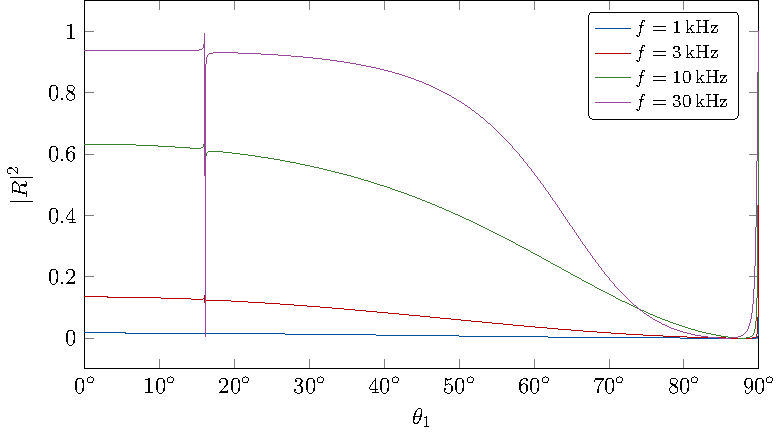
\includegraphics[width=\textwidth]{../../LaTeX/createFigures/TikzFigures/raytracing_PhD/absRVStheta_1}
	\caption{Reflection coefficient for steel plate ($h=\SI{8}{mm}$) in water}
	\label{Fig:absRVStheta_1}
\end{figure}
\begin{figure}
	\centering
	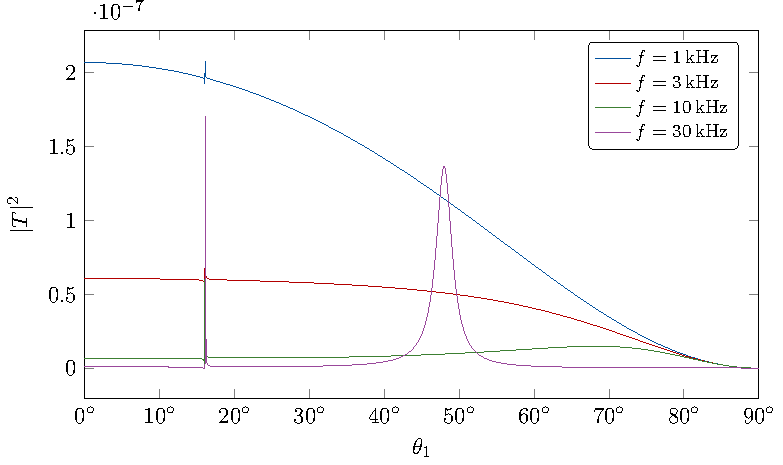
\includegraphics[width=\textwidth]{../../LaTeX/createFigures/TikzFigures/raytracing_PhD/absRVStheta_2}
	\caption{Transmission coefficient for steel plate ($h=\SI{20}{mm}$) between water and air}
	\label{Fig:absRVStheta_2}
\end{figure}
The coefficients in~\Cref{Tab3:BeTSSiCoeffs1,Tab3:BeTSSiCoeffs2} can be used as an approximation (for all $\theta_1$) if the above formulas become too cumbersome to evaluate when simulating the BeTSSi models.
\begin{table}
	\centering
	\caption{Transmission and reflection coefficients for a steel shell of thickness $h=\SI{20}{mm}$ with water in layer 1 and air in layer 3 at $\theta_1=0$.}
	\label{Tab3:BeTSSiCoeffs1}
	\begin{tabular}{S[table-format = 2.0] S[table-format = -1.9,round-mode=places,round-precision=9] S[table-format = -1.9,round-mode=places,round-precision=9] S[table-format = -1.9,round-mode=places,round-precision=9] S[table-format = -1.9,round-mode=places,round-precision=9]}
		\toprule
		$f~[\si{kHz}]$ & {$\Re T$} & {$\Im T$} & {$\Re R$} & {$\Im R$}\\
		\hline
1 & 0.000379766969018 & 0.000249718630540 & -0.395896148267406 & -0.917881662236952\\
3 & 0.000111196929936 & 0.000219612051919 & 0.591993752825717 & -0.805804333434816\\
10 & 0.000012214011183 & 0.000081497140085 & 0.956075958461063 & -0.293076431782431\\
30 & 0.000001289902104 & 0.000029417561237 & 0.996162572651329 & -0.087503949282425\\
		\bottomrule
	\end{tabular}
\end{table}
\begin{table}
	\centering
	\caption{Transmission and reflection coefficients for a steel shell of thickness $h=\SI{8}{mm}$ with water on both sides of shell at $\theta_1=0$.}
	\label{Tab3:BeTSSiCoeffs2}
	\begin{tabular}{S[table-format = 2.0] S[table-format = -1.9,round-mode=places,round-precision=9] S[table-format = -1.9,round-mode=places,round-precision=9] S[table-format = -1.9,round-mode=places,round-precision=9] S[table-format = -1.9,round-mode=places,round-precision=9]}
		\toprule
		$f~[\si{kHz}]$ & {$\Re T$} & {$\Im T$} & {$\Re R$} & {$\Im R$}\\
		\hline
1 & 0.982994356142675 & 0.129425410351553 & 0.0170056082885165 & -0.129158693991996\\
3 & 0.865266600396151 & 0.34183851179542 & 0.134733079454665 & -0.341038325402061\\
10 & 0.366032205988348 & 0.483053260835384 & 0.633964233015312 & -0.480384557030005\\
30 & 0.059738859577007 & 0.241054268607891 & 0.940228789459313 & -0.233010582837406\\
		\bottomrule
	\end{tabular}
\end{table}